\chapter{Endogenous taxation in ongoing internal conflict: The case of Colombia}\footnote{This chapter was coauthored with Jacob Shapiro (Princeton University), Abbey Steele (University of Amsterdam) and Juan F. Vargas (Universidad El Rosario). The chapter was published in the American Political Science Review in 2018, Volume 112, Issue 4, pp. 996 - 1015.} 

\section{Introduction}

Historically, conflicts have motivated states to develop their fiscal capacity. According to \citet{tilly92a}, the formation of nation-states in early modern Europe emerged in part by the fiscal demands created by expansionary external wars. Those demands incentivized leaders to develop institutions that could monitor local populations and levy taxes. The resulting tax revenue was used to finance armies that would protect their kingdoms from external threats or expand their territories. Subsequent work provides empirical support for this theory at the cross-country level \citep{besleypersson08a} and refines it for regions outside of Europe \citep{centeno03a, vu10b} and for more recent time periods \citep{schevestasavage12a}.\footnote{Despite broad support for the theory, some have challenged its validity for early modern Europe \citep[e.g.,][]{spruyt96a, ertman97a, gorski93a}.} 

Yet the effect of \textit{internal} wars on statebuilding and fiscal capacity is more ambiguous. While an extension of Tilly's logic to internal wars implies that the state should try harder to state-build when challenged, that clearly does not always happen. This rasies an important question: what prevents would-be contemporary state-builders from acting on these incentives? Of course, when two parties are seeking to build competing tax institutions within the same territory (e.g. state and rebels), then the net effect is ambiguous. \citet{centeno03a} also argues that the prevalence of civil wars rather than mass wars in Latin America accounts for the weaker states in the region, because they fostered elite divisions, physical destruction and military rather than mass mobilization. 

Empirically, \citet{besleypersson08a} and \citet{cardenaseslava14a} provide evidence that internal conflict negatively affects various measures of state capacity. In Southeast Asia, however, \citet{slater10a} finds that communal urban unrest and endemic violence are both likely to lead elites to tax themselves. And in Latin America, \citet{soifer15a} finds evidence that the prevalence of conflict was crucial for extending the state during the 19\textsuperscript{th} century, and \citet{rodriguez-franco16a} finds that Colombia's elites in Bogot\'{a} began  to support statebuilding through new taxes in the early 2000s after several decades of internal conflict.  
  
The literature has so far focused on national-level fiscal capacity, but contemporary states feature multiple administrative layers, and a critical ingredient for the consolidation of the state is the introduction of sound and efficient tax systems at the local level. Moreover, security provision, property rights protections and a variety of development projects at the local level could, in theory, facilitate state-building by shaping citizens' preferences and behavior in ways that favor the state over its competitors. 

Several potential mechanisms have been proposed to explain the relationship between internal conflict and state capacity that are relevant for thinking about the relationship between conflict and tax performance at the local level. To mention a few: (1) By destroying physical capital, inducing forced migration and reducing the market value of private property in affected areas, conflict deteriorates the tax base; (2) Conflict generates negative reciprocity of tax payers towards a state that they judge to have failed to protect them \citep{cardenaseslava14a}; (3) A conflict environment reduces the return of productive activities and raise that of illegal businesses, which do not pay taxes to the state \citep{besleypersson08a}; (4) Armed groups create their own governance systems that divert civilians' resources away from the state and crowd out state institutions \citep{mampilly11a, arjona16a, sanchez-de-la-sierra17a}; and (5) Conflict facilitates the emergence of interest groups with {\it de facto} power (for instance because of their access to weapons) that can capture local political and economic institutions \citep{eaton06a, lopez10a, mampilly11a}. Such capture prevents state institutions from eliminating competitors, and from creating a durable and credible relationship with citizens in these regions.

We focus on the latter political economy mechanism. In the context of internal conflicts local tax institutions (both formal and informal) are shaped by different types of vested interests. We explore the extent to which armed groups shape existing property and tax institutions \textit{differently} depending on their preferences. To the best of our knowledge, this mechanism has not been studied in the previous literature, either theoretically or empirically.\footnote{See \citet{eaton06a} and \citet{lopez10a} on other forms of capture by illegal armed groups in Colombia. \citet{mampilly11a} analyzes rebel governance more broadly and \citet{arjona14a} finds that armed groups operated alongside state institutions in roughly one-quarter of the Colombian communities in her sample.} Our argument is that local tax and property rights institutions are shaped by illegal armed actors who influence state institutions to further their interests and those of the civilian groups they favor. Specifically, we expect that right-wing paramilitary groups will favor establishing formal property rights for land owners, while left-wing insurgents will do the opposite.

We test this argument in Colombia, which has four traits that make it an ideal setting for studying the relationship between civil conflict, institutional capture and local tax performance. First, the dynamics of the internal conflict vary substantially across the country's 1,122 municipalities. Moreover, within each municipality violence also varies across different periods of the war.  Second, Colombia sits roughly in the middle of the distribution of non-OECD countries in terms of the share of tax revenues generated locally \citep{deMello2000}.\footnote{The share of tax revenue collected locally is the standard measure of revenue decentralization in the literature, but is only available for a limited subset of countries.} It also ranks in the middle of large developing countries in terms of local revenue mobilization, above Indonesia at ~38\% but below India at approximately 62\% \citep{bird2012}. Third, local government authorities have substantial freedom to shape property and tax institutions. They can choose tax rates, order or impede updates on the land value, select revenue collection methods, and alter penalties and incentives. In theory, this autonomy could facilitate efficient local tax administration by allowing the system to be tailored to the needs of each municipality. In practice, in the context of uneven state presence and varying degrees of contestation by illegal armed groups, local institutions can be captured by private groups with vested interests.\footnote{This insight follows naturally from the theory in \citet{perssontabellini02a}, among others, in which heterogeneous agents take advantage of the discretion granted them.} 

Fourth, and most importantly, the main combatants had clear preferences regarding state-backed property rights throughout much of the war, which had implications for the local tax base and performance. Right-wing paramilitaries favored land owners, and promoted the accumulation of large estates which served as means to launder illegally acquired capital (through the drug trade, for example) or realize economies of scale in agricultural production and cattle ranching \citep{reyes07a}.\footnote{Paramilitaries displaced people to take their land and titling in areas with paramilitary presence was not always above-board. For example, public notaries, the officials charged with validating the provenance of land, were infiltrated by paramilitaries \citep[e.g.,][]{duran12a, verdad-abierta12a}.} 
On the left-wing side, both FARC and ELN guerrilla groups aimed to replace what they characterized as an unjust state and claimed to be acting on behalf of peasants and workers. The guerrillas backed land invasions of state and private property in many areas \citep[e.g.,][]{steele17a}. The FARC also viewed state-recognized private property as illegitimate or unnecessary: in its VIII Conference in 1993, it still backed collectivized property \citep{bernal-morales14a}. (During peace talks with the Santos administration in 2012, the FARC supported land formalization for the first time.) In areas that they influenced, the guerrillas regulated property in parallel to the state. For instance, they claimed the right to redistribute unused land or land from narcotraffickers \citep{bernal-morales14a}.\footnote{Internal divisions with the FARC existed, but it was a centralized organization that adopted policies in its Conferences that were relatively well enforced throughout. The paramilitaries were more decentralized but none challenged the basic legitimacy of state institutions (even if they argued that they could be run more effectively) \citep{gutierrez-sanin08a,romero03a}.} 

These positions on property rights stem from ideological commitments and make sense from the perspective of combatants trying to maximize their control over territory, and to mobilize supporters. Historically, land titling and formalization has favored the wealthy and powerful in Colombia \citep{albertuskaplan13a, flores14a}, and the FARC issued its own tax rules. By obstructing the formal property rights regime, the FARC could meet its ideological commitments, impede the state in territory where it had influence, and avoid double taxing residents. Paramilitaries, on the other hand, were supported by groups such as large land owners who benefit from formal titles, including to secure land acquired through violence and coercion.\footnote{Early paramilitary supporters included drug traffickers who purchased vast tracts of land \citep{romero00a, ronderos14a}.} The fact that formal titles create an obligation to pay local property taxes would be a relatively small price to pay to secure new property.

In Colombia, we can make these expectations concrete and test them using disaggregated information on local institutions.  We constructed a novel municipal-level dataset that includes information on various dimensions of property and tax institutions, including the land value recorded in the cadaster (i.e. property registry), the number of cadastral updates, and the duration between updates.\footnote{The cadaster and the property title registry (\textit{Registro de Instrumentos P\'{u}blicos}) form the basis for property rights. The cadaster records the physical characteristics of land plots and properties, such as the size and value. The Registro records the title holder for the property. As part of the peace agreement with the FARC, a new integrated cadaster and registro is planned, to eliminate red tape and modernize the cadaster. See \citet{departamento-nacional-de-planeacion16a}.} Municipal taxes are primarily levied on property value, which is recorded and updated in the cadaster. Cadaster updates are supposed to occur every five years, but municipal administrations are responsible for initiating and paying for the update and a high proportion do not meet this legal obligation \citep{departamento-nacional-de-planeacion16a}. These data allow us to observe property and tax institutions at a high resolution. We combine these data with administrative information on municipal property tax revenues as well as with variables that account for the longitudinal dynamics of conflict activity in Colombia.

We find that armed groups' violent activity correlates with differences in property formalization and taxation that are consistent with the groups' political positions. Municipalities with significant insurgent violence report less land formalization and lower tax receipts. Municipalities that experienced significant paramilitary violence have more land formalization and higher tax receipts. Revenue changes are mirrored by changes in socio-economic outcomes, including development levels (measured with nighttime light intensity) as well as secondary school enrollment, which are higher in areas with more paramilitary violence and lower in areas with more guerrilla violence.

There are three obvious mechanisms which could drive the relationship between violence and revenue: (1) indirect capture through intimidation and pressure on political actors to update or not the cadaster; (2) direct capture of institutions through elections of favored candidates who then carry out the policy preferred by the armed group; and (3) reductions in tax revenues due to violence hurting the economy and by extension, property value. The last of these is unlikely because it implies symmetric effects of violence by the two parties on revenue, which we do not see. Turning to (1) and (2), though we cannot directly measure intimidation and pressure, we can measure electoral outcomes. Municipalities with more paramilitary violence do have a greater probability of electing candidates from former President Uribe's right-wing political party coalition, while the probability decreases in municipalities with high guerrilla violence. Causal mediation analysis, however, shows that little of the relationship between violence and tax revenue works through electoral outcomes: the causal mediation effect is small, statistically insignificant, and close to zero. This leads us to believe that more indirect mechanisms of capture, such as threats and violence against mayors and city council representatives, account for the differences in tax revenue and land formalization across municipalities. 

Overall then, guerrilla and paramilitaries' asymmetric influence on tax performance and land formality are consistent with armed group capture at the local level. The higher the level of violence by an armed group, the more tax institutions' outcomes shift in the direction of that group's preferences.

This paper contributes to our understanding of contemporary state-building during internal wars in four ways. First, our findings show that armed groups have the ability to capture the state's local institutions to shape policy outcomes in their favor, which can block the state from developing effective institutions. Though \citet{centeno03a} argues that a minimal administrative state is a necessary condition to generate state-building in Tilly's framework, we show that capture is an overlooked concern even when this condition is met. Second, we offer evidence that armed groups' preferences and civilian ``constituencies'' are relevant for how they behave \citep{wood03a, gutierrez-sanin03a}. Third, the variation in how armed groups reshape local tax institutions in their favor implies a need for a disaggregated approach to post-conflict reconstruction. In Colombia, for example, the state should focus on land redistribution and progressive taxation measures in areas where the paramilitaries were dominant. In areas where insurgents were dominant, attention to land formalization and tax collection should be prioritized. Finally, there is a broader policy lesson in these results. While fiscal decentralization might maximize political economy goals in stable countries, it may also engender significant drawbacks in those experiencing ongoing violence \citep{steeleschubiger15a, eaton06a}. To restore the state's control over local tax institutions and property rights, the central state may have to limit municipal autonomy. 
 
The rest of the paper is organized as follows: the next section provides some context and discusses the theoretical framework of our argument. This is followed by the introduction of the data sources and our empirical strategy. The subsequent section presents the main results and robustness checks, followed by the conclusion to the article.

\section{Context}

\subsection{Tax institutions and tax performance in Colombia}

Municipalities in Colombia vary widely in their tax performance. Figure \ref{chapter3_fig:taxrevenues} plots the ratio of tax revenue to total expenditure (averaged for the period 2000-2012) across the country's 1,122 municipalities. The average municipality levies taxes worth 12\% 
of their expenditure, with the balance supplied by transfers from the national government based on population size and poverty levels, as well as royalties from natural resource extraction. The variation is enormous, with several municipalities unable to generate practically any revenue and a few capable of financing up to 80 percent of their expenditures with local taxes. 

\begin{figure}[H]
\begin{center}
\caption{Tax revenue over total expenditure across Colombian municipalities}
\label{chapter3_fig:taxrevenues}
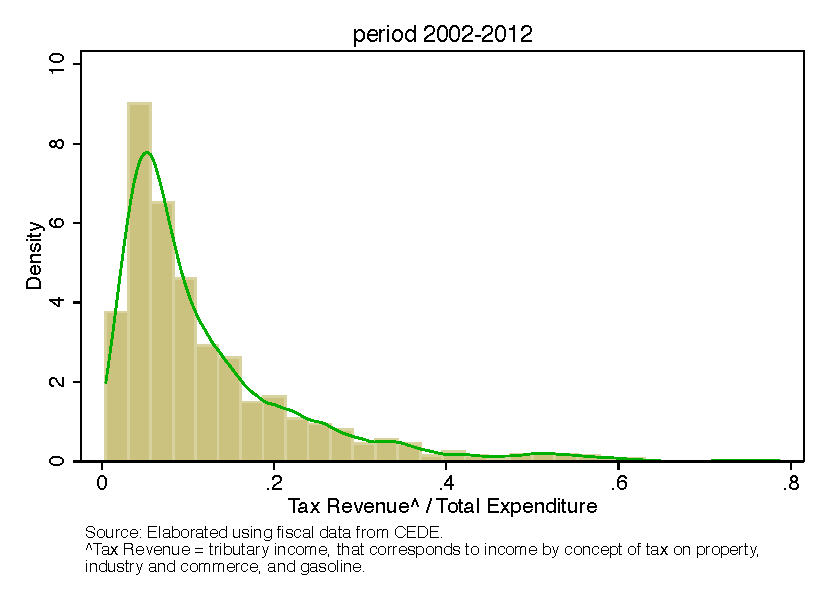
\includegraphics[width=1\textwidth]{Chapter3/Figures/figure1.pdf}
\end{center}
\end{figure}

The variation is not simply a proxy for economic activity, as Figure \ref{chapter3_fig:distributionrevenues} shows. Panel A plots the distribution of different tax revenues per capita at the municipal level, averaged from 2000 to 2012.\footnote{Tax revenues are in constant Colombian pesos from 2008.} Panel B shows the same results normalized using nighttime lights to proxy for economic activity \citep{vernon11}. The first column presents logged tributary income while the second shows the distribution of logged property tax income, which comprises the bulk of local revenue.\footnote{Both are logged given their highly skewed distributions, with a long right tail of municipalities with larger tributary and property tax income.} 

The large variation in tax receipts reflects the freedom that local authorities have in designing tax institutions. While the municipal mayor (the highest local-level executive authority) is in charge of updating the land registry, the city council (the municipal legislative body) issues the municipality's tax statute, which includes the tax rates, the type of properties for which each rate applies, the collection methods, and the payment incentives and fines.\footnote{As stated above, the cadaster is supposed to be updated every five years, but mayors are responsible for initiating the process. Then the national geographic institute, Instituto Geogr\'afico August\'in Codazzi (IGAC), is supposed to carry out the actual update with municipal resources. Although the municipal council sets tax rates, they must fall within a range defined by the National Congress. The current range for property tax is 5-16 per thousand for all types of properties. \citet{nunez05a} reviews Colombia's local tax system.} Property tax rates vary substantially between rural and urban areas, and may or may not vary by type of property or its specific use (e.g. private housing, production, or commercial purposes). In addition, systems can be mixed within municipalities, with some properties and businesses taxed according to one rule (e.g. the value of the property recorded in the municipal cadaster), and others according to another (e.g., the socioeconomic conditions of the neighborhood where the properties are located). The majority of municipalities have mixed systems that combine various schemes.

\begin{figure}[H]
\begin{center}
\caption{Tax revenue across Colombian municipalities, by type}
\label{chapter3_fig:distributionrevenues}
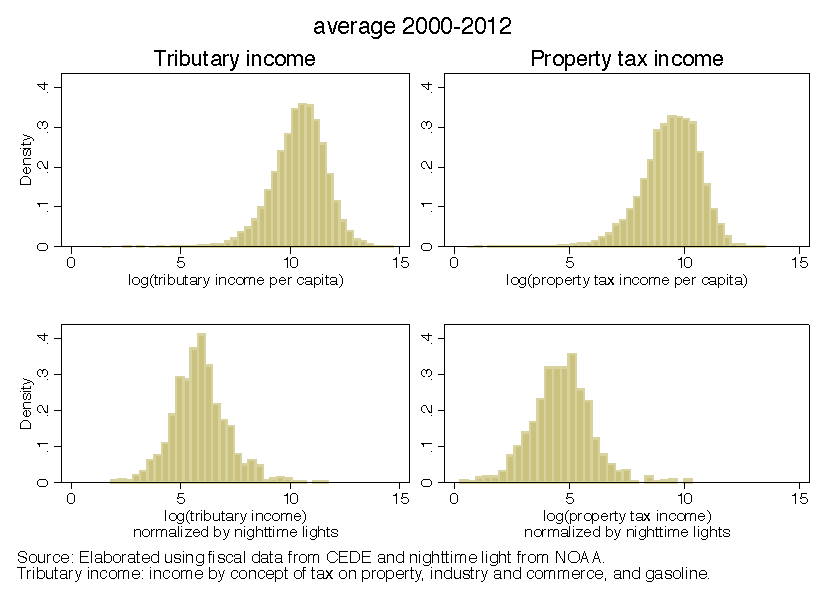
\includegraphics[width=1\textwidth]{Chapter3/Figures/figure2.pdf}
\end{center}
\end{figure}

Regardless of the tax rates and system, the cadaster forms the basis of property taxes.\footnote{Some residents pay property taxes even in the absence of formal title, because it is a way to demonstrate continual presence on a parcel of land. According to Colombian law, investments in land that make it ``socially productive'' can be rewarded with formal property rights for the land in question after five consecutive years of residence (Law 200 of 1936).} The cadaster includes the property values and the physical traits of properties. Outdated cadasters reduce the amount of revenue a municipality collects in property taxes, because recorded property values are lower than the true values \citep{iregui-b.b.04a}. 

\subsection{The capture of local tax and property institutions}

In Latin America, only Brazil and Venezuela have more decentralized systems, and in the rest of the countries in the region, provincial or national governments are in charge of tax legislation. In Colombia, fiscal autonomy was pursued because policymakers thought that it, combined with other decentralization reforms, could help end the war \citep[534, 541]{eaton06a}. The Betancur administration (1982-1986) approved the direct election of mayors that began in 1988, and the two subsequent administrations under Barco and Gaviria devolved fiscal authority and budgetary responsibility to municipalities for several public goods such as education, health, and road upkeep. 

Unfortunately, despite those changes (and partly as a result of them), the civil war intensified and spread in the 1990s \citep{sanchezmar-palau06a, steeleschubiger15a,steele17a}. Municipalities became attractive targets for armed groups because of the transfers and royalties they received and because the state was insufficiently equipped to provide security to them. \citet[537]{eaton06a} writes, ``...the state now funds its own destabilization because armed groups on the left and right have been able to appropriate decentralized public revenues and to use these funds to further reduce the state's already limited monopoly over the use of force.'' The influence of armed groups over locally elected politicians could be substantial.   

In Colombia, insurgents and right-wing paramilitary groups differed in their approaches to capture the state \citep{lopez-hernandez10a, eaton06a, 07a}. Paramilitary groups frequently colluded with state forces, but were independent of them. They forged extensive ties to regional- and national-level politicians \citep[16]{gutierrez-sanin10c}. Indeed, paramilitaries were embraced, and, in some cases, even founded by the country's regional political elites \citep{romero03a, ronderos14a, duncan06a}.  

In contrast, the FARC focused on local organization, particularly through the Juntas de Acci\'{o}n Communal (JACs), committees based in the rural hamlets within municipalities. While the FARC also engaged with some municipal-level and national-level officials, they did so to a far lesser extent then the paramilitaries.\footnote{For example, in 2010 only 10 of the 277 alcaldes and municipal council members under investigation for ties to illegal armed groups were linked to the FARC; similarly, only 4\% of the congress was investigated for ties to the FARC, compared to 35\% to paramilitary groups \citep[33]{lopez-hernandez10a}.} As \citet[18-19]{gutierrez-sanin10c} points out, insurgents are less reliable partners for politicians, because they are anti-state. Consistent with their leftist ideology, insurgents tried to mobilize and work with peasants and workers who were traditionally shut out of the political system.  The distinct ``constituencies'' of insurgents and paramilitaries imply differing preferences over policies.

A particularly fraught policy area that armed groups intervened in is land formalization, which has implications for local tax performance. Right-wing paramilitaries were founded by large landowners and narco-traffickers who began to purchase tracts of land. As they expanded, they displaced peasants and claimed their land \citep{romero00a, ronderos14a, reyes09a}. To legitimate this transfer of land, paramilitaries sought to formalize property through the state. This was consistent with what we noted above: traditionally, elites have been able to secure legal title to their property, while poor peasants face multiple barriers to doing so. Updating cadasters to reflect newly acquired or changed properties (for instance, an enlarged plot of land) is consistent with an interest in securing property rights, even if the property is illegally acquired (for instance through claiming the land of a displaced household).\footnote{\citet{ibanezmunoz11a} find that the concentration of land between 2000 and 2009 increases as the result of an increase in plots and an increased number of plots purchased by few people.} 

Left-wing insurgents favored more equitable land distribution but not private property rights \citep{bernal-morales14a}. One way they promoted this goal was through land invasions, where poor peasants and workers would occupy state lands (\textit{bald\'{i}os}) or private property. However, such invasions were typically not formalized legally. More common in insurgent areas was a preference for excluding or prohibiting representatives of the state from surveying the land or plotting the property -- necessary steps in the formalization process.\footnote{Corporaci\'on Regional para el Desarrollo Sostenible del Area de Manejo Especial la Macarena (CORMACARENA) official interview with the authors, Vista Hermosa, 26 January 2011. This official told us he could not conduct land surveys in the area because the FARC would not permit it.}  

Given the divergent preferences of and incentives for armed groups to shape local property institutions, we expect differences in local property tax performance overall. We propose four hypotheses:

\begin{quotation}
In areas with substantial FARC and ELN violence: 

\noindent $H_{1a}$ Tax revenues per capita will be lower because fewer properties will be formalized.

\noindent $H_{1b}$ Left wing parties will tend to outperform in mayoral and municipal council elections controlling for the pre-existing partisan balance.

\bigskip
In areas with substantial paramilitary violence:

\noindent $H_{2a}$ Tax revenues per capita will be higher because more property will be formalized. 

\noindent $H_{2b}$ Right wing parties will tend to outperform in mayoral and municipal council elections controlling for the pre-existing partisan balance.
\end{quotation}

Though we expect tax revenue to be higher in areas with paramilitary presence, and lower in areas with insurgent presence, we do not argue that right-wing paramilitaries or the elites that supported them favored increased taxation, or that the left-wing insurgents opposed redistribution. Instead, armed groups' preferences over tax rates and enforcement are ambiguous in Colombia. Paramilitaries might try to benefit supporters by pushing for lower rates and lax enforcement of property taxes. This position would be consistent with historical precedent in the 20th century: \citet{sanchez-talanquer18a} finds that following large-scale land reform attempts, local elites registered property in the cadaster to establish their property rights, but manipulated property value to avoid paying higher tax. At the same time, paramilitaries could benefit from an increase in local tax revenue because they issued lucrative contracts to supporters to carry out municipal functions like health services \citep{eaton06a, verdad-abierta15b}.\footnote{Though ideally we could test the effects of armed groups' influence on tax rates and enforcement, we do not have the data to do so. In the end what we do test is the net effect of their influence on local property tax revenue. These data indicate that whatever is happening with tax rates and enforcement, land formalization measures increase tax revenue overall.} New landowners could also calculate that paying taxes was a small cost to pay for securing property, and employ tax resources to expand their control over the local bureaucracy and bargaining power relative to higher levels of government \citep{sanchez-talanquer18a,pardelli2018}. Moreover, short-term development of specific local administrative capacities does not prevent the long-term hollowing out and capture of the state in Colombia \citep{stasavage2014}. 
%[[AS: I cut this segment because it made it difficult for me to follow: "to consolidate their power by pushing wages downward to control labor mobility, while"; also changed "privatization" of the state to "capture."]]

Insurgents, though they did favor redistribution, preferred not to work through the state's institutions because doing so would legitimate the state. The FARC issued its own tax code, targeting the wealthy in areas of their influence (see below). In terms of property rights, the insurgents preferred to impede the efforts of the state \citep{bernal-morales14a} and regulate land on its own.\footnote{One example of the FARC's intransigence on state-backed property rights was its opposition to land restitution for the internally displaced through the Victims Law of 2011, calling it ``legal dispossession'' \citep{bernal-morales14a}.}  

Before we explain how we test our hypotheses, we first summarize temporal trends in capture over the course of the war. 
	
\subsection{Civil war dynamics and capture in Colombia}

The dynamics of the civil war in terms of territorial control and violence have changed significantly over time. We separate the war's recent evolution, and the armed groups' capture strategies, into four periods and organize the statistical analysis around these four periods because pooling them would effectively assume that armed actors had the same ability to influence tax policies in every year, which strikes us as substantively unrealistic. The four periods (described in detail in Appendix H) can be defined as follows: 

\begin{itemize}

\item \textbf{1988-1996: FARC ascendancy}. 
According to one estimate the FARC went from a presence in 173 of the country's municipalities in 1985 to 622 by 1995 \citep[28]{echandia06a}. 
By the end of the period, the FARC and the ELN both enforced election boycotts in areas under their control, and threatened elected mayors and local council members \citep{el-tiempo97a}. 
While some regional politicians supported paramilitaries' formation during this period \citep[37]{ronderos14a}, there is little evidence that paramilitary groups tried to capture political institutions directly at the local level during this period.

\item \textbf{1997-2002: Paramilitary expansion}. 
In 1997, regional paramilitary groups united under the umbrella group United Self-Defense Forces of Colombia (AUC) and the war spread. By 2001, the AUC was powerful enough to convene a meeting with nearly 100 politicians to formulate a concerted effort to win elections at all levels, and to support \'Alvaro Uribe's candidacy for president in 2002 (known as the Santa Fe de Ralito pact). Compared to the paramilitaries, the FARC's influence remained indirect during this period as the group eschewed official electoral politics during this period, preferring to threaten municipal candidates that the group did not approve of, or acting mayors.

\item \textbf{2003-2006: Paramilitary demobilization}.
In 2003, the Uribe administration negotiated a ceasefire with paramilitary groups and eventually adopted the `Justice and Peace' law, allowing paramilitary commanders to demobilize their troops in exchange for lenient sentences. Paramilitary demobilizations from 2003 to 2005 transformed the war into a contest between the state and remaining insurgent groups (the FARC and ELN). The conflict with the FARC continued apace during this period, with no change in their capture strategy.

\item \textbf{2007-2010: State resurgence}.
Having pushed the FARC into peripheral areas by the end of 2006, the Colombian military and police redeployed to major population centers and roads, improving measures of security. The weakened FARC agreed to peace talks following the 2010 election of Uribe's Minister of Defense, Juan Manuel Santos. Former paramilitary groups morphed into new organizations---including the ``Black Eagles,'' and drug-trafficking groups such as the ``Urabe\~{n}os'' and the ``Rastrojos'' — which sometimes engaged in actions against the FARC, the ELN, and the civilian population, though at much lower rates than in previous times.

\end{itemize}

Taking into account these time periods, Figure \ref{chapter3_fig:violence_revenues} shows the department-level relationship between cumulative attacks by armed group and average property tax revenues in the following time period.\footnote{There are 32 departments in Colombia. This administration level is equivalent to US states.} There are two main takeaways: first, departments in Colombia vary widely in the correlation between tax performance and the type and level of armed group presence; second, and following the historical shifts of the Colombian war, this variation changes over time, a feature that will be exploited in the empirical specification to test our hypotheses, and in the substantive interpretation of results.\footnote{Correlations are carried out at the department level since municipalities are the lowest administrative unit in our data.}

\medskip


\begin{figure}[H]
\begin{center}
\caption{Relationship between property tax revenues and attacks per armed group and time period across Colombian departments}
\label{chapter3_fig:violence_revenues}
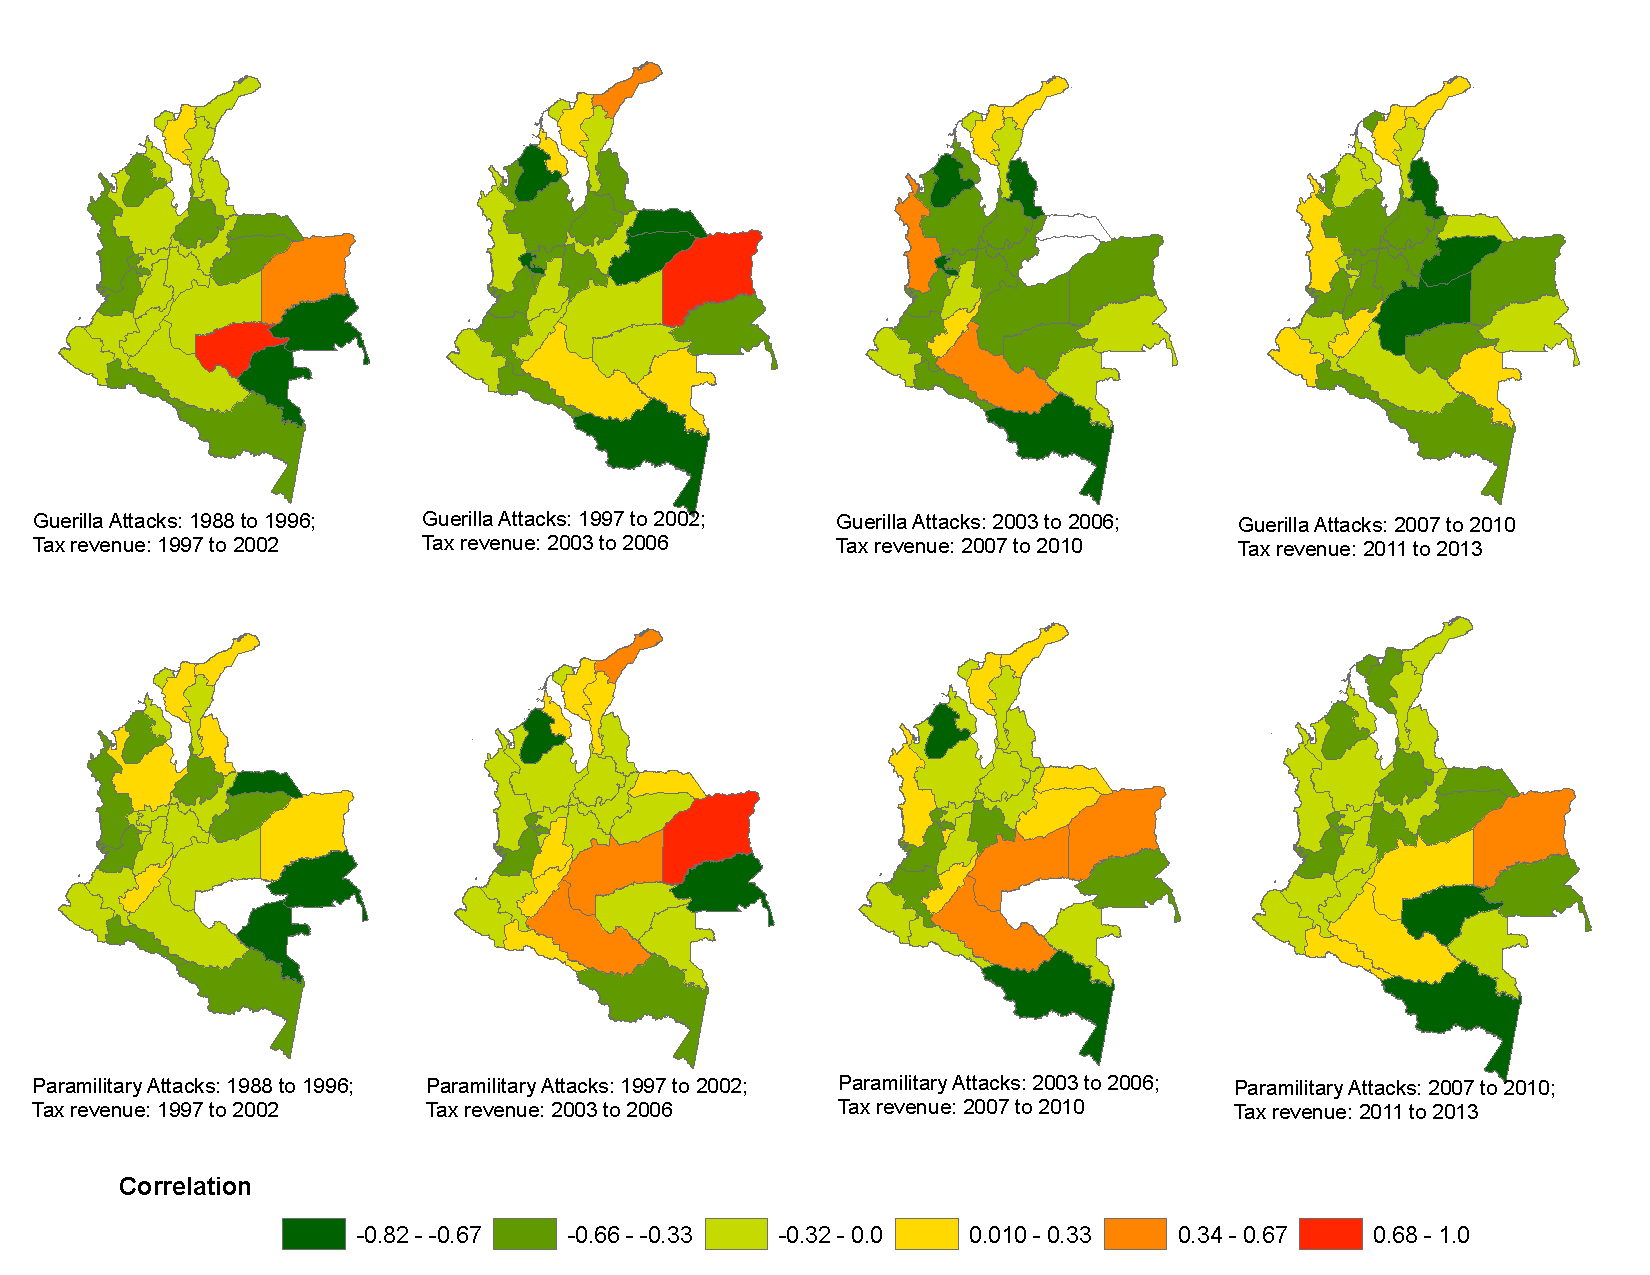
\includegraphics[width=1\textwidth]{Chapter3/Figures/figure3.pdf}
\end{center}
\end{figure}
Notes: Violence data from the Human Rights Observatory of the Office of the Vice-President, Colombia, and fiscal data from CEDE. Revenues are average property tax receipts by specified time period. Attacks are cumulative attacks per 100,000 inhabitants per armed group, by specified time period. 

\subsection{Data}

Table \ref{chapter3_tab:descriptive} provides descriptive statistics of our main outcome variables, used to test both the main empirical relationships and the mechanisms described in our testable hypotheses (Panel A). Outcomes include logged tax revenues per capita, proxies of cadastral performance, the land informality rate and electoral outcomes. Tax revenues are highly skewed, with a long right tail of municipalities with substantially greater tax revenues per capita than others.\footnote{The wealthiest municipalities had tax receipts as much as ten standard deviations above the mean.} We therefore run our estimation of the impact of violence on property tax revenues per capita on logged values.\footnote{The results are substantially the same when we add to the set of controls the log of the municipal population instead of using per capita tax revenue.}

Table \ref{chapter3_tab:descriptive} also describes the independent variables of interest (Panel B), namely the cumulative attacks perpetrated by each of the two main armed groups, during each one of the four periods that mark the evolution of Colombia's civil war, as described in the ``Civil War Dynamics and Capture in Colombia'' section.\footnote{See the Appendix \ref{data_appendix3} for detailed descriptions of all the variables and measures.} Measuring the influence exercised by an armed group over a specific location is extremely challenging. Indicators of presence and non-violent coercion over a large set of municipalities cannot be systematically recorded in an objective way. Violence, on the other hand, while more easily observed, is only imperfectly correlated with territorial dominance. For instance, it may be the case that municipalities with low levels of violence or no armed contestation represent an armed group stronghold, where tax policies are likely to be influenced.

%%-----------------------------------------------------------%

% Table 1 Descriptive Stats

\begin{table}[h]
\centering 
\caption{Descriptive statistics of main variables}
\label{chapter3_tab:descriptive}
\scalebox{0.65}{
\begin{tabular}{l c c c c c}\hline\hline
\multicolumn{1}{c}{\textbf{Variable}} & \textbf{Mean}
 & \textbf{Std. Dev.}& \textbf{Min.} &  \textbf{Max.} & \textbf{N}\\ \hline
 \\
 \multicolumn{6}{c}{Panel A. Outcomes} \\

{\it Tax revenues per capita}	&		&		&		&		&		\\ 

Log property tax revenues per capita 1997-2002&        2.32&        1.08&           0&           6&        1108\\
Log property tax revenues per capita 2003-2006&        2.70&        1.00&           0&           6&        1107\\
Log property tax revenues per capita 2007-2010&        2.82&        1.06&           0&           6&        1111\\
Log property tax revenues per capita 2011-2013&        2.94&        1.11&           0&           7&        1111\\




\\
{\it Cadastral performance}	&		&		&		&		&		\\ 

Per capita land value 2003-2006&        4.60&        5.79&           0&          79&         974\\
Cadastral update lag 2003-2006&        6.82&        3.87&           0&          50&         892\\
Num. cadastral updates 2003-2006&        1.49&        0.67&           0&           4&         979\\



\\
{\it Land ownership}	&		&		&		&		&		\\ 

Land informality rate 2003-2006&        0.20&        0.23&           0&           1&         954\\

\\
{\it Electoral outcomes}	&		&		&		&		&		\\ 

Uribe + Conservative party coalition 1997 Mayor election&        0.28&        0.45&           0&           1&         986\\
Uribe + Conservative party coalition 2000 Mayor election&        0.26&        0.44&           0&           1&         955\\
Uribe + Conservative party coalition 1997 and 2000 Mayor elections&        0.32&        0.46&           0&           1&        1182\\
Uribe + Conservative party coalition 2003 Mayor election&        0.23&        0.42&           0&           1&         908\\
Uribe + Conservative party coalition 2007 Mayor election&        0.60&        0.49&           0&           1&        1106\\
Uribe + Conservative party coalition 2003 and 2007 Mayor elections&        0.61&        0.49&           0&           1&        1182\\
Uribe + Conservative party coalition 2011 Mayor election&        0.43&        0.50&           0&           1&        1040\\


\\
 \multicolumn{6}{c}{Panel B. Violence} \\

Log guerrilla attacks per capita, 1988-1996&      -35.42&       31.30&        -115&           0&        1182\\
Log paramilitary attacks per capita, 1988-1996&      -35.87&       31.53&        -105&           0&        1182\\
Log guerrilla attacks per capita, 1997-2002&      -29.38&       19.80&         -82&           0&        1182\\
Log paramilitary attacks per capita, 1997-2002&      -30.02&       20.04&         -74&           0&        1182\\
Log guerrilla attacks per capita, 2003-2006&      -18.12&       12.67&         -53&           0&        1182\\
Log paramilitary attacks per capita, 2003-2006&      -19.61&       14.10&         -53&           0&        1182\\
Log guerrilla attacks per capita, 2007-2010&      -13.94&       13.07&         -48&           0&        1182\\
Log paramilitary attacks per capita, 2007-2010&      -16.49&       15.73&         -55&           0&        1182\\
Log guerrilla attacks per capita, 2003-2010&      -32.06&       23.73&        -101&           0&        1182\\
Log paramilitary attacks per capita, 2003-2010&      -36.10&       27.71&        -108&           0&        1182\\



\hline \hline
\multicolumn{6}{p{1.4\textwidth}}{\footnotesize{Notes: All data sources are described in Appendix \ref{data_appendix3}.}} \\
\end{tabular}
}
\end{table}

However, non-violent dominance is unlikely to occur without any violence inflicted in the past, either as a way to legitimize influence with the citizenry or to oust any contesting (legal or illegal) group. It is thus reasonable to assume that the ability to inflict localized violence over a relatively long period could be expected to translate into influence in different ways. Moreover, as all our results are robust to controlling for violence by the other actor, we posit that municipalities with greater violence are more likely to be captured by the perpetrating armed group.\footnote{A more stringent test is to focus on the subsample of places where violence by both groups is recorded, dropping the municipalities where one group does not engage in any violence at all during the sample period. Even with the statistical power reduction implied by the limited sample, Appendix D shows that out main results are robust to this exclusion.}

We thus follow a growing empirical literature on the Colombian conflict (see e.g. \citet{acemoglurobinson13a}, \citet{fergussonetal2016} and \citet{fergussonetal2018}) and use a past stock measure of violence over a period of years as an (imperfect) indicator of influence. \citet{arjonaotalora11a} compare existing databases of civil war violence in Colombia to survey evidence on armed groups' presence (for the small subsample of municipalities for which the latter is available) and conclude that while violence is likely to {\it underestimate} --by roughly the same magnitude- both guerrilla and paramilitary control, there is a non-negligible correlation between both measures.\footnote{The authors do not use cumulative past violence, hence the correlation of survey-based presence indicators with our proposed measure is probably larger.} 

To further validate our proposed measure of armed groups' influence, we report the correlations between groups' cumulative attacks and other (group-specific) proxies of presence. The recent peace agreement signed by the Colombian government and FARC in September 2016 was followed by the demobilization of over 10,000 FARC combatants in the so called {\it Espacios Territoriales de Capacitaci\'on y Reincorporaci\'on}, ETCR (Spanish for territorial areas of training and reincorporation). The ETCR are located in 25 of the municipalities of FARC's highest historical influence. The correlation between an ETCR indicator and cumulative guerrilla attacks of the last conflict period we study (2007 - 2010) is 0.3 (significant at the 1\% level). Instead, the correlation of ETCR with cumulative paramilitary attacks is 0.09. Similarly, following a DDR process with the government of \'{A}lvaro Uribe (see ``Civil War and Capture in Colombia'' section, several paramilitary units adding up to over 35,000 ex-combatants) demobilized in 36 municipalities where, arguably, their dominance was high. The correlation between an indicator of these municipalities and cumulative paramilitary attacks over the period 1997 - 2002 is 0.1, and significant at the 1\% level. Instead, the correlation with cumulative guerrilla attacks is 0.02, and not significant.\footnote{For all the above reasons, we believe that violence is an imperfect but valid proxy of armed influence. But even if it was not, the strong relationship of violence to changes in local fiscal institutions that we document in this paper is an important fact that has not been previously documented, and that should inform our thinking on how conflict influences state building and development.}

Similar to the case of tax revenues, attacks by guerrilla fronts and paramilitary blocks are highly skewed, especially in the 1988-2010 period (see also Figure \ref{chapter3_fig:map}). The most violent municipalities had attacks over eight standard deviations above the mean. We thus normalize attacks by population so as to capture violence intensity, and use logged values in the regressions (since normalized variables remain highly skewed).\footnote{The statistical significance of the results below becomes weaker when using a log-linear model with unlogged violence per-capita, with t-statistics in the 1.3-1.6 range, though all results retain the same sign. This means that the results are surely not driven by outliers in attacks, as logging the per capita attack variable effectively attenuates those observations' influence on the estimates.}

\begin{figure}[H]
\begin{center}
\caption{Guerrilla and paramilitary attacks across Colombian municipalities}
\label{chapter3_fig:map}
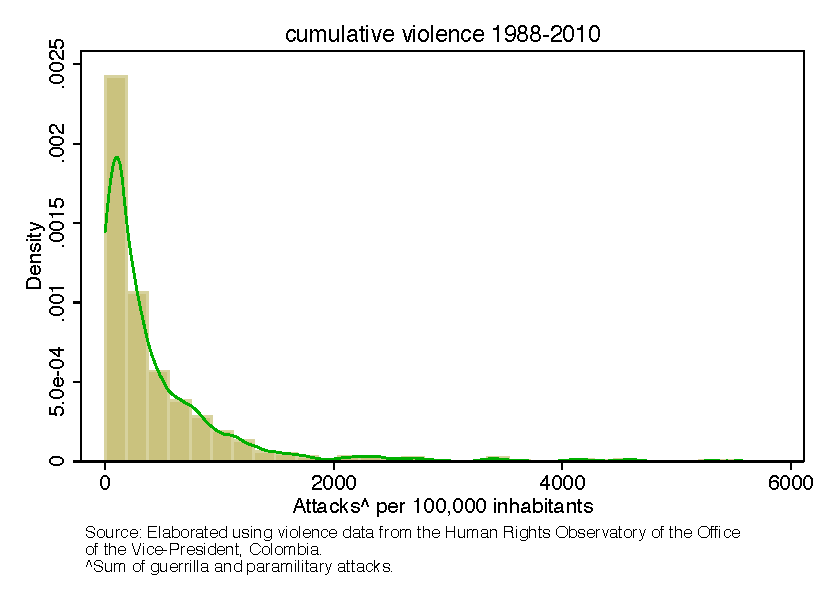
\includegraphics[width=1\textwidth]{Chapter3/Figures/figure4.pdf}
\end{center}
\end{figure}

Appendix \ref{data_appendix3} provides a detailed description of both the main and all the additional variables (summarized in Table \ref{appendix3:description_vars}). All of our specifications control for a large set of municipal-level potential confounders, including natural resource royalties and transfer payments, vote share by political party for mayors' elections, the location of military bases, a dummy of `peaceful' municipalities (those without attacks during our entire sample period), the number of people displaced due to the armed conflict, coca production and municipal geographic characteristics. We also control for a resources-endowment additive index, that includes the production of gold, silver, platinum, nickel and iron.\footnote{Note that some of these variables are potentially {\it bad controls} as they can respond to cumulative past violence. In the ``Additional Robustness Checks'' subsection we discuss this issue and show that our results are not affected by post-treatment bias.} 


\subsection{Estimation} 

Because the modern internal conflict in Colombia had four distinguishable periods with their own intensity and dynamics, as summarized in the subsection on ``Civil War Dynamics and Capture in Colombia'', we test how violence-related capture during each specific period correlates with local tax performance during the subsequent period. We examine lagged outcomes both because tax institutions cannot shift overnight and because studying the relationship between conflict events within a given period and tax institutions immediately after that period minimizes simultaneity problems. 

Running a standard panel data approach with municipality and time fixed-effects would entail two untenable assumptions: (1) that the conditional impact of violence on taxes operates in the short term; and (2) the treatment effect of influence (as proxied by violent incidents) is the same in every period. Both seem substantively problematic. On (1), tax institutions are slow to change, in part because mayors and council member have a 3 or 4 year office period (depending on if before or after 2003) and they update the cadaster and the rates once in that period, if anything. On (2), the intensity of violence varied significantly across periods, so fitting a model that assumes constant marginal effects of violence on outcomes would be incorrect. 

We therefore estimate an OLS specification at the municipality level separately for each of the periods mentioned above. With tax revenue, for example, we estimate:

		\begin{align}
			\label{eq:revenue}
			\mbox{Tax Revenue}_{i,t} = \alpha + \gamma_d+  \beta_1 \mbox{Cum. Guerrilla Attacks}_{i,(t-\Delta \text{ to } t-1)} \nonumber \\ 
			+ \beta_2 \mbox{Cum. Paramilitary Attacks}_{i,(t-\Delta \text{ to } t-1)} + \Phi \mathbf{X}_{i,t} + \epsilon_{i,t} \\ \forall \ t \in \{(1997 \text{ to } 2002), (2003 \text { to } 2006), (2007 \text { to } 2010), (2011 \text{ to } 2013) \nonumber \}
		\end{align}
\noindent where 	 	
 $\mbox{Tax Revenue}_{i,t}$ is the log property tax revenue per capita in a municipality, $i$, in a given period, $t$, after each of the described violence periods;\footnote{We report multiple post-treatment years to explore potential cumulative effects.} $ \mbox{Cum. Guerrilla Attacks}_{i,(t-\Delta \text{ to } t-1)}$ and $\mbox{Cum. Paramilitary Attacks}_{i,(t-\Delta \text{ to } t-1)}$ capture logged total attacks per capita that accumulate over each period described in the subsection ``Civil War Dynamics and Capture in Colombia'' subsection, and preceding $t$; $\mathbf{X}_{i,t}$ is a vector of municipality-level control variables as described in the previous subsection.\footnote{Municipal-level production of coca is available only since 1999. Our post 1999 results are robust to adding this variable in the vector $\mathbf{X}_{i,t}$. We address potential concerns regarding the inclusion of post-treatment controls explicitly below.} We also include a Department fixed-effect, $\gamma_d$, to account for any department-level time-invariant heterogeneity across each of the 32 second-level administrative units, the next level administrative unit up from the municipality. 
We are thus working off within-department variation in violence, controlling for a range of geographic factors. Hence, our estimates account for the {\it excess} tax revenue in municipalities that experience more violence by one party or the other above the department mean. We report robust standard errors throughout, clustered at the department level.\footnote{We believe this to be a conservative approach. If we follow \citet{acemoglurobinson13a} by simply using robust standard errors all results become somewhat stronger statistically.}

Our identifying assumption with this approach is that levels of violence during each period of the internal conflict were conditionally independent of future tax revenues. Our controls are grounded in the rich literature on civil war, which cites incentives for capture and the advantages (or disadvantages) of terrain as key determinants of contestation. One concern with this approach is that we could simply be picking up enduring cross-sectional within-department differences, correlated both with the presence of different armed groups as well as with the trajectory of tax revenues. To rule this out we include a set of regressions controlling for tax revenue in the municipality at the end of the period prior to each period in which cumulative violence is measured ($\mbox{Tax Revenue}_{i,t-\Delta-1}$ in the notation above). When estimating the partial correlation of tax revenue from 2003-6 with violence from 1997-2002, for example, we include a specification controlling for tax revenues in 1993-1996, and so forth with the other time periods.

\section{Results}

\subsection{Violence and tax revenue}

As a first glance at armed groups' influence on tax institutions, we use specification (1) to estimate the relationship between cumulative past violent activity by armed groups and property tax revenue. As shown in Table \ref{chapter3_tab:main}, we find that violence perpetrated by guerrillas is consistently negatively associated with property tax revenue, while violence by paramilitaries is positively correlated with it. 

Table \ref{chapter3_tab:main} focuses on four different time periods. Columns 1 and 2 show the relationship between logged total violence per capita from 1988-1996 on average logged tax revenues per capita in 1997 through 2002. Columns 3 and 4 show the relationship between violence in 1997-2002 and tax revenues in 2003 through 2006. Columns 5 and 6 show the relationship between violence in 2003-2006 and tax revenues in 2007 through 2010. Lastly, columns 7 and 8 show the relationship between violence in 2007-2010 and tax revenues from 2011 to 2013, the last period we have data for. 

%%-----------------------------------------------------------%
%

% Table 2. Main Table
\newpage

%\begin{landscape}
\begin{table}[htbp]\def\sym#1{\ifmmode^{#1}\else\(^{#1}\)\fi}
\caption{Cumulative violence and property tax performance}
\label{chapter3_tab:main}
\begin{center}
\scalebox{0.65}{
\begin{tabular}{lcccccccc}

\hline \hline 
\multicolumn{9}{l}{Dependent variable: {\it Log of property tax revenue per capita} over period:}\\


&\multicolumn{2}{c}{1997-2002}              &\multicolumn{2}{c}{2003-2006}              &\multicolumn{2}{c}{2007-2010}              &\multicolumn{2}{c}{2011-2013}              \\\cmidrule(lr){2-3}\cmidrule(lr){4-5}\cmidrule(lr){6-7}\cmidrule(lr){8-9}
            &\multicolumn{1}{c}{(1)}         &\multicolumn{1}{c}{(2)}         &\multicolumn{1}{c}{(3)}         &\multicolumn{1}{c}{(4)}         &\multicolumn{1}{c}{(5)}         &\multicolumn{1}{c}{(6)}         &\multicolumn{1}{c}{(7)}         &\multicolumn{1}{c}{(8)}         \\
\addlinespace
\begin{tabular}[c]{@{}l@{}}Log guerrilla attacks\\ per capita \underline{1988-1996}\end{tabular}&     -0.0746\sym{***}&     -0.0384\sym{***}&                     &                     &                     &                     &                     &                     \\
            &    (0.0087)         &    (0.0073)         &                     &                     &                     &                     &                     &                     \\
\addlinespace
\begin{tabular}[c]{@{}l@{}}Log paramilitary attacks\\ per capita \underline{1988-1996}\end{tabular}&      0.0715\sym{***}&      0.0367\sym{***}&                     &                     &                     &                     &                     &                     \\
            &    (0.0089)         &    (0.0072)         &                     &                     &                     &                     &                     &                     \\
\addlinespace
\begin{tabular}[c]{@{}l@{}}Log guerrilla attacks\\ per capita \underline{1997-2002}\end{tabular}&                     &                     &     -0.0951\sym{***}&     -0.0318\sym{**} &                     &                     &                     &                     \\
            &                     &                     &    (0.0090)         &    (0.0100)         &                     &                     &                     &                     \\
\addlinespace
\begin{tabular}[c]{@{}l@{}}Log paramilitary attacks\\ per capita \underline{1997-2002}\end{tabular}&                     &                     &      0.0903\sym{***}&      0.0302\sym{**} &                     &                     &                     &                     \\
            &                     &                     &    (0.0095)         &    (0.0104)         &                     &                     &                     &                     \\
\addlinespace
\begin{tabular}[c]{@{}l@{}}Log guerrilla attacks\\ per capita \underline{2003-2006}\end{tabular}&                     &                     &                     &                     &     -0.0708\sym{***}&     -0.0173\sym{*}  &                     &                     \\
            &                     &                     &                     &                     &    (0.0130)         &    (0.0082)         &                     &                     \\
\addlinespace
\begin{tabular}[c]{@{}l@{}}Log paramilitary attacks\\ per capita \underline{2003-2006}\end{tabular}&                     &                     &                     &                     &      0.0643\sym{***}&      0.0137\sym{+}  &                     &                     \\
            &                     &                     &                     &                     &    (0.0123)         &    (0.0077)         &                     &                     \\
\addlinespace
\begin{tabular}[c]{@{}l@{}}Log guerrilla attacks\\ per capita \underline{2007-2010}\end{tabular}&                     &                     &                     &                     &                     &                     &     -0.0655\sym{*}  &     -0.0120         \\
            &                     &                     &                     &                     &                     &                     &    (0.0248)         &    (0.0074)         \\
\addlinespace
\begin{tabular}[c]{@{}l@{}}Log paramilitary attacks\\ per capita \underline{2007-2010}\end{tabular}&                     &                     &                     &                     &                     &                     &      0.0472\sym{*}  &      0.0078         \\
            &                     &                     &                     &                     &                     &                     &    (0.0219)         &    (0.0067)         \\
\addlinespace
Observations&         986         &         986         &        1070         &        1070         &        1107         &        1107         &        1107         &        1107         \\
R-squared   &       0.533         &       0.672         &       0.565         &       0.754         &       0.542         &       0.818         &       0.531         &       0.874         \\
Controls$^a$&  \checkmark         &  \checkmark         &  \checkmark         &  \checkmark         &  \checkmark         &  \checkmark         &  \checkmark         &  \checkmark         \\
Depto. FE   &  \checkmark         &  \checkmark         &  \checkmark         &  \checkmark         &  \checkmark         &  \checkmark         &  \checkmark         &  \checkmark         \\
Pre-period tax revenue$^b$&                     &  \checkmark         &                     &  \checkmark         &                     &  \checkmark         &                     &  \checkmark         \\



\hline \hline
\multicolumn{9}{p{1.35\textwidth}}{\footnotesize{Notes: Standard errors in parentheses are clustered at the department level; Significance-level: $^{***}$ 0.1\%; $^{**}$ 1\%; $^*$ 5\%; and $^{+}$ 10\%, refers to two-sided t-tests. Outcome measured in constant 2008 Colombian pesos.
$^a$ Controls include: royalties and transfers per capita, municipality area, elevation, distance to the department's capital, vote share by political party ideology, dummy variable on whether the municipality had no registered homicides in the same period as the attacks  (independent variables), the number of military bases, the number of people displaced, driven out and received by municipality due to conflict, average coca production, and an additive endowment index on the production of gold, silver, platinum, nickel, emeralds and iron.%
$^b$ Estimations include the pre-period property tax revenue per capita, i.e. the period from 1985 to 1987 in column (2), from 1993 to 1996 in (4), from 2000 to 2002 in (6), and from 2003 to 2006 in (8), to pick up part of the enduring cross-sectional within-department differences. }} \\
\end{tabular}
}
\end{center}
\end{table}
%\end{landscape}

Odd columns show that guerrilla attacks are negatively correlated with tax revenues, a relationship that is statistically significant across the four periods. In contrast, cumulative past paramilitary attacks are positively correlated with tax revenues in every period. Even columns show that the results for the first three conflict periods are robust to controlling for pre-period tax revenues. Statistical significance is however attenuated in the last period. This is consistent with the observation that paramilitary groups officially demobilized from 2003 to 2006 (largely becoming criminal bands), and guerrilla groups were weakened from 2007 to 2010 (see section on ``Civil War Dynamics and Capture in Colombia''). Thus, we would not expect the effects to be as strong in the third and especially the fourth period. This effectively turns the last period into a {\it placebo}.\footnote{Figure \ref{chapter3_fig:figure5} is the graphical counterpart of Table \ref{chapter3_tab:main} (even columns). We plot the point estimates as well as the 95\% confidence intervals, documenting that the estimated effects decrease overtime. The differences across conflict periods are not statistically significant, with the exception of the comparison between the first and the fourth period. Again, as expected, during the state resurgence period, point estimates lean towards zero.} 

\begin{figure}[H]
\begin{center}
\caption{Estimated relationship between property tax revenues and attacks per armed group and time period across Colombian municipalities}
\label{chapter3_fig:figure5}

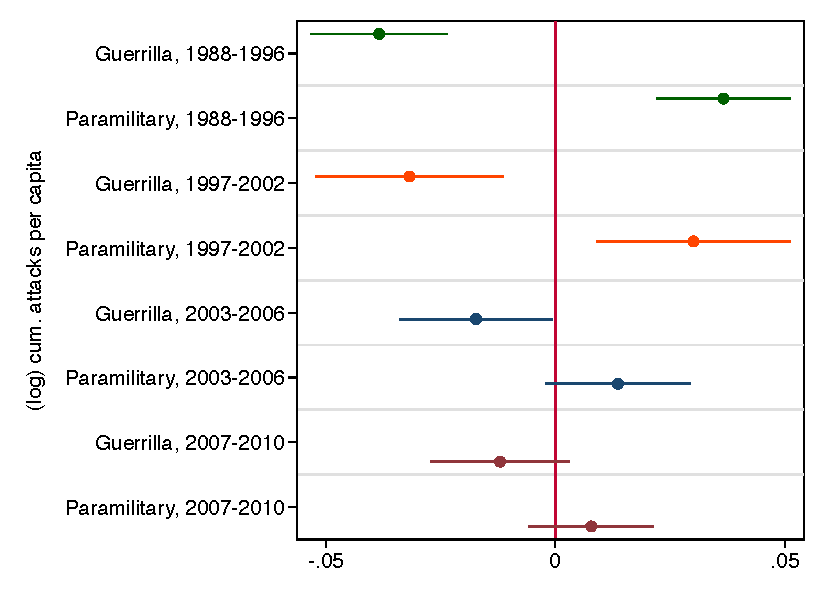
\includegraphics[width=1\textwidth]{Chapter3/Figures/figure5.pdf}
\end{center}
\end{figure}
Notes: Regression estimates from Table \ref{chapter3_tab:main}, columns (2), (4), (6), and (8), respectively. Treatment variables in logs as specified in Table \ref{chapter3_tab:main}.  


Because of the log-log specification, estimated coefficients should be interpreted as the elasticity of per capita property tax revenue with respect to cumulative past violence. Given the estimated elasticities we can compute substantive effects by multiplying them with changes of interest in the independent variable (expressed in terms of percent changes). Using the most demanding specification in column 2 of Table \ref{chapter3_tab:main}, an increase in cumulative per capita guerrilla attacks (paramilitary attacks) over the period 1988-1996 from the median to the 90$^{th}$ percentile of the distribution is associated with an average 37\% drop (13\% increase) in per capita property tax income over the period 1997-2002. An equivalent increase in cumulative violence in the period 1997-2002 is associated with a 16\% drop, and a 11\% increase, in per capita property tax income over the period 2003-2006 for the case of guerrilla and paramilitary attacks, respectively (column 4). Further,  
An equivalent increase in cumulative violence in the period 2003-2006 is associated with a 20\% drop, and a 8\% increase, in per capita property tax income over the period 2007-2010 for the case of guerrilla and paramilitary attacks, respectively (column 6).\footnote{Figure \ref{chapter3_fig:margins} reports the marginal-effect plots of the effect of cumulative past guerrilla and paramilitary violence on property tax revenues, with a horizontal axis support ranging from the median to the 90$^{th}$ percentile.}

\begin{figure}[H]
\begin{center}
\caption{Cumulative violence (1997-2002), tax revenues, and potential mechanisms (2003-2006): change in predictions from the median to the 90$^{th}$ percentile}
\label{chapter3_fig:margins}
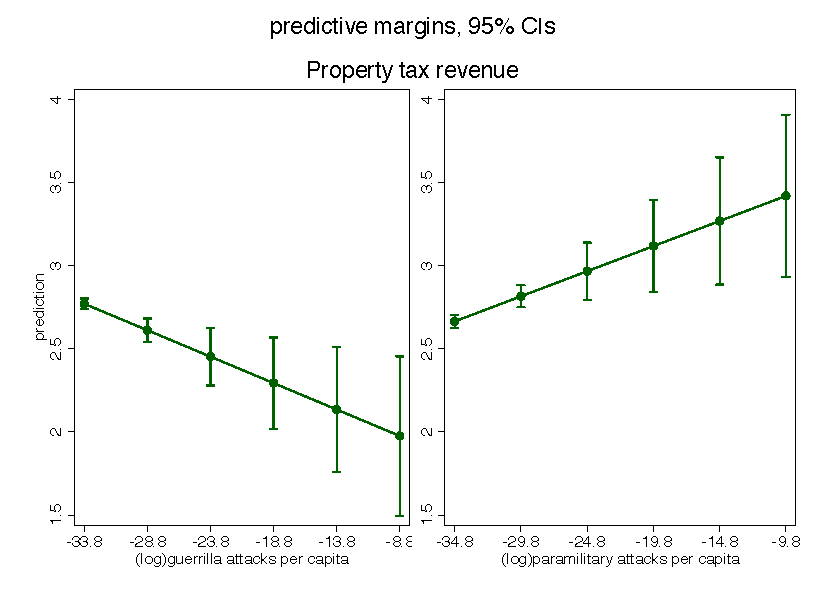
\includegraphics[width=.75\textwidth]{Chapter3/Figures/figure6_part1.pdf}
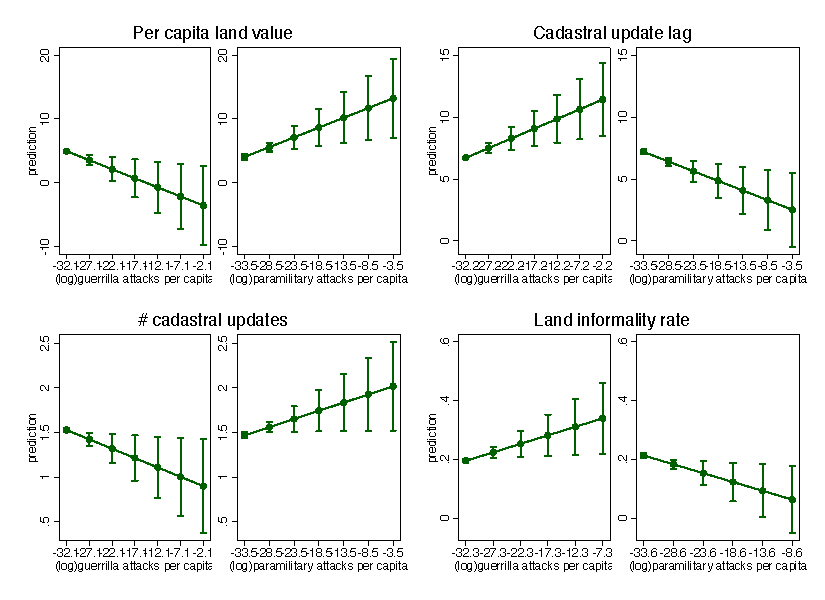
\includegraphics[width=1\textwidth]{Chapter3/Figures/figure6_part2.pdf}
\end{center}
Note: Elaborated using Table \ref{chapter3_tab:main}, second period, and \ref{chapter3_tab:table3} estimates.
\end{figure}

\subsection{Robustness}

While our four conflict periods are based on our substantive theoretical and historical understanding of the evolution of the Colombian civil war, a potential concern is that the results reported in Table \ref{chapter3_tab:main} are just an artifact of an arbitrary aggregation of annual data into these periods. Appendix E shows that this is not the case. We re-run our most demanding empirical specification (including pre-period tax revenues) using year-by-year moving windows in which six (eight) years of cumulative conflict are correlated with three (five)-year aggregations of tax revenues.

Figures \ref{appendix3:moving_window_6years} and \ref{appendix3:moving_window_8years} report the results graphically, respectively for the six and the eight-year moving windows. In both cases, we corroborate the asymmetric correlation of guerrilla and paramilitary cumulative past violence of municipal tax performance. Also consistent with our main results (Table \ref{chapter3_tab:main}) and with the historical account of the conflict (section ``Civil War Dynamics and Capture in Colombia''), Figures \ref{appendix3:moving_window_6years} and \ref{appendix3:moving_window_8years} suggest that armed groups' influence decreases in the later periods, especially for the case of paramilitaries.

\subsection{Implications}
Appendix \ref{appendix3:why_matters} analyzes the implications of the influence that armed groups exert on tax revenues, both for a set of education outcomes that respond to municipal-specific investments and for a proxy of municipal-specific economic performance. Tables \ref{appendix3:consequences_violence} and \ref{appendix3:consequences_economic} suggest that cumulative past guerrilla violence is associated with less human capital accumulation and poor economic performance, respectively. The opposite is true for paramilitary activity.

\subsection{Mechanisms: Tax Institutions and Land Formalization}

What explains the association between violence and tax performance, and particularly the heterogeneity across different armed groups? We expect that a key channel is through land formalization.
 
Recall that the mayor is in charge of managing and updating the land registry, and the city council can decide tax rates, tax collection mechanisms, enforcement, and fines. Since either or both these government levels can be captured by violent groups with vested interests, we explore two things: first, the extent to which the intensity of the internal conflict is correlated with variation in outcomes associated with the responsibilities of both the local authorities related to land formalization and taxation; and second, the extent to which armed groups captured local authorities through electoral outcomes.

Table \ref{chapter3_tab:table3} uses the empirical specification in \eqref{eq:revenue} to estimate the effect of cumulative past guerrilla and paramilitary violence on potential mechanisms related to the functioning of municipal tax institutions and land formalization. In particular, we look at land value (columns 1 and 2), the time elapsed since the last cadastral update (columns 3 and 4), the number of cadastral updates carried out by a municipality (columns 5 and 6) and the share of properties that lack land titles (columns 7 and 8). 

%---------------------------------------
% Table 3. Mechanisms

%\begin{landscape} 
\begin{table}[htbp]
\def\sym#1{\ifmmode^{#1}\else\(^{#1}\)\fi}\caption{Mechanisms: Cumulative violence (1997-2002) and potential mechanisms (2003-2006)}
\label{chapter3_tab:table3}
\begin{center}
\scalebox{0.65}{
\begin{tabular}{lcccccccc}
\hline \hline 
  & (1) & (2) & (3) & (4) & (5) & (6) & (7) & (8)   \\
 \hline 
 \\  

&\multicolumn{2}{c}{\emph{Per capita land value}}&\multicolumn{2}{c}{\emph{Cadastral update lag}}&\multicolumn{2}{c}{\emph{\# cadastral updates}}&\multicolumn{2}{c}{\emph{Land informality rate}}\\\cmidrule(lr){2-3}\cmidrule(lr){4-5}\cmidrule(lr){6-7}\cmidrule(lr){8-9}
\addlinespace
\begin{tabular}[c]{@{}l@{}}Log guerrilla attacks\\ per capita \underline{1997-2002}\end{tabular}&     -0.5266\sym{***}&     -0.2841\sym{*}  &      0.1988\sym{***}&      0.1568\sym{**} &     -0.0315\sym{**} &     -0.0210\sym{*}  &      0.0139\sym{***}&      0.0058\sym{*}  \\
            &    (0.1414)         &    (0.1045)         &    (0.0435)         &    (0.0496)         &    (0.0089)         &    (0.0090)         &    (0.0026)         &    (0.0025)         \\
\addlinespace
\begin{tabular}[c]{@{}l@{}}Log paramilitary attacks\\ per capita \underline{1997-2002}\end{tabular}&      0.5386\sym{***}&      0.3064\sym{**} &     -0.1967\sym{***}&     -0.1557\sym{**} &      0.0284\sym{**} &      0.0183\sym{*}  &     -0.0137\sym{***}&     -0.0060\sym{*}  \\
            &    (0.1455)         &    (0.1077)         &    (0.0456)         &    (0.0515)         &    (0.0084)         &    (0.0087)         &    (0.0025)         &    (0.0024)         \\
\addlinespace
Observations&         939         &         939         &         867         &         867         &         942         &         942         &         927         &         927         \\
R-squared   &       0.361         &       0.445         &       0.293         &       0.298         &       0.450         &       0.462         &       0.515         &       0.574         \\
Controls$^a$&  \checkmark         &  \checkmark         &  \checkmark         &  \checkmark         &  \checkmark         &  \checkmark         &  \checkmark         &  \checkmark         \\
Depto. FE   &  \checkmark         &  \checkmark         &  \checkmark         &  \checkmark         &  \checkmark         &  \checkmark         &  \checkmark         &  \checkmark         \\
Pre-period tax revenue$^b$&                     &  \checkmark         &                     &  \checkmark         &                     &  \checkmark         &                     &  \checkmark         \\


\hline \hline
\multicolumn{9}{p{1.3\textwidth}}{\footnotesize{Notes: Standard errors in parentheses are clustered at the department level; Significance-level: $^{***}$ 0.1\%; $^{**}$ 1\%; $^*$ 5\%; and $^{+}$ 10\%, refers to two-sided t-tests. $^a$ Controls as in Table \ref{chapter3_tab:main}.
$^b$ Due to the lack of 1993-1996 data for these dependent variables, regressions include pre-period property tax revenue per capita from 1993 to 1996 in (2), (4), (6), and (8) to pick up part of the enduring cross-sectional within-department differences.
}} \\
\end{tabular}
}
\end{center}
\end{table}
%\end{landscape}

Consistent with our main results, cumulative past guerrilla violence is negatively correlated with land value and the number of cadastral updates, and positively correlated with the cadastral update lag and with land informality rate. Paramilitary violence has exactly the opposite correlation signs with these variables, and these results are robust to controlling for the pre-period tax revenue (even columns). Overall, these results suggest that guerrillas favor informal land arrangements that keep state institutions at bay, and help peasants avoid formal taxes. In contrast, the evidence suggests that paramilitaries favor the formal land arrangements that large land owners prefer. 
 
Taking into account the log-level nature of the specifications reported on Table \ref{chapter3_tab:table3}, the substantive magnitude of the estimated coefficients can be computed by multiplying them with changes of interest in the independent variable (expressed in terms of percent changes) and dividing the product by 100. Using the specification of column 2, an increase in cumulative per capita guerrilla (paramilitary) attacks over the period 1997-2002 from the median to the 90$^{th}$ percentile of the distribution is associated with an average drop (increase) of 24\% (19\%) of a standard deviation in average per capita land value over the period 2003-2006. Similarly, the same increase in cumulative per capita guerrilla violence is associated with little over three quarters of a year delay in updating the local land cadaster. In turn, the equivalent increase in paramilitary violence is associated with a decrease in the cadastral update lag of just over half a year (column 4). The number of cadastral updates carried out in the municipality drops (increases) by 15\% (10\%) of a standard deviation when guerrilla (paramilitary) attacks over the period 1997-2002 increase from the median to the 90$^{th}$ percentile (column 6). Finally, an equivalent change in cumulative past guerrilla (paramilitary) violence is associated with an increase (decrease) of 12\% (9\%) of s standard deviation of the municipal land informality rate over the period 2003-2006 (column 8).\footnote{Figure \ref{chapter3_fig:margins} reports marginal-effect plots for these four outcomes. The horizontal axes include values of our violence measures ranging from the median to the 90$^{th}$ percentile. In all cases, the asymmetry of the correlation of cumulative past guerrilla violence and that perpetrated by paramilitaries is evident.}


\subsection{Mechanisms: Electoral outcomes}

The asymmetric relationship between levels of insurgent and paramilitary violence and outcomes related to both property tax revenue and land formality support a mechanism of institutional capture. Given that local authorities set property tax rates, armed groups might try to exercise influence in two ways: indirectly through intimidation, or directly by getting preferred candidates elected. Specifically, given the authority that municipal councils have to set property tax rates, we would expect armed groups to try to influence council members, and the local council elections towards their favored candidates. In addition, the mayor has the responsibility to update the cadaster, so mayoral elections could be similarly vulnerable to armed groups' influence. 
We test these implications with data on electoral results for election years 1997, 2000, 2003, 2007, and 2011. 

First, we study whether the probability that a candidate from President Uribe's right-wing political party coalition wins a mayor's election is greater in places with higher past cumulative paramilitary violence, and lower in places with more guerrilla violence. Results are reported on Table \ref{chapter3_tab:table4}, Panel A.\footnote{Alternatively we can look at the vote share of the Uribe coalition in mayoral elections. This is indeed the approach followed for the city council elections (Table 6, Panel C), as the existence of several council seats makes the winning dummy approach inappropriate for this context. For completeness, we show the correlation between cumulative past violence and the vote share of Uribe's coalition in mayoral elections in Panel B.} Because Uribe was first elected President in 2002, we aggregate the 1997 and 2000 election results (when no Uribe coalition existed). The null results for these elections (columns 1 and 2) are thus expected, and can be interpreted as a falsification test.\footnote{These null results also hold if we estimate the same model for both election years separately (results available upon request).} We also aggregate the third and fourth periods described in the subsection on ``Civil War Dynamics and Capture in Colombia'', given that the 2003 and 2007 local elections occurred in the middle of Uribe's administration (2002-2010).\footnote{Again, the results are robust to treating both election years separately.} Both in the case of the 2003-2007 elections (columns 3 and 4), as well as in the 2011 elections (columns 5 and 6), places with higher guerrilla past cumulative violence experience a decrease in the probability that a candidate from Uribe's coalition wins a mayoral election. Instead, in places with higher levels of past paramilitary violence, that probability is higher.

%-----------------------------------------------------------%

% Table 4. Mechanisms: Direct capture, Cumulative violence and Electoral Outcomes 

%\begin{landscape}
\begin{table}[htbp]
\def\sym#1{\ifmmode^{#1}\else\(^{#1}\)\fi}\caption{Mechanisms: Direct capture, Cumulative violence and electoral outcomes}
\label{chapter3_tab:table4}
\begin{center}
\scalebox{0.65}{
\begin{tabular}{lcccccc}
\hline \hline 
\multicolumn{7}{l}{Dependent variable: {\it Uribe Coalition + Conservative Party} }\\
& \multicolumn{6}{c}{Panel A: {\bf Win dummy, Mayor Election$^a$}} \\ 

&\multicolumn{2}{c}{1997 and 2000 Elections}&\multicolumn{2}{c}{2003 and 2007 Elections}&\multicolumn{2}{c}{2011 Election}          \\\cmidrule(lr){2-3}\cmidrule(lr){4-5}\cmidrule(lr){6-7}
            &\multicolumn{1}{c}{(1)}         &\multicolumn{1}{c}{(2)}         &\multicolumn{1}{c}{(3)}         &\multicolumn{1}{c}{(4)}         &\multicolumn{1}{c}{(5)}         &\multicolumn{1}{c}{(6)}         \\
\addlinespace
\begin{tabular}[c]{@{}l@{}}Log guerrilla attacks\\ per capita \underline{1988-1996}\end{tabular}&      0.0007         &      0.0033         &                     &                     &                     &                     \\
            &    (0.0044)         &    (0.0035)         &                     &                     &                     &                     \\
\addlinespace
\begin{tabular}[c]{@{}l@{}}Log paramilitary attacks\\ per capita \underline{1988-1996}\end{tabular}&      0.0011         &     -0.0025         &                     &                     &                     &                     \\
            &    (0.0046)         &    (0.0038)         &                     &                     &                     &                     \\
\addlinespace
\begin{tabular}[c]{@{}l@{}}Log guerrilla attacks\\ per capita \underline{1997-2002}\end{tabular}&                     &                     &     -0.0113\sym{+}  &     -0.0123\sym{*}  &                     &                     \\
            &                     &                     &    (0.0061)         &    (0.0058)         &                     &                     \\
\addlinespace
\begin{tabular}[c]{@{}l@{}}Log paramilitary attacks\\ per capita \underline{1997-2002}\end{tabular}&                     &                     &      0.0135\sym{*}  &      0.0140\sym{*}  &                     &                     \\
            &                     &                     &    (0.0063)         &    (0.0059)         &                     &                     \\
\addlinespace
\begin{tabular}[c]{@{}l@{}}Log guerrilla attacks\\ per capita \underline{2003-2010}\end{tabular}&                     &                     &                     &                     &     -0.0073\sym{+}  &     -0.0085\sym{*}  \\
            &                     &                     &                     &                     &    (0.0038)         &    (0.0038)         \\
\addlinespace
\begin{tabular}[c]{@{}l@{}}Log paramilitary attacks\\ per capita \underline{2003-2010}\end{tabular}&                     &                     &                     &                     &      0.0084\sym{**} &      0.0093\sym{**} \\
            &                     &                     &                     &                     &    (0.0030)         &    (0.0030)         \\
\addlinespace
Observations&        1040         &        1040         &        1041         &        1041         &         900         &         900         \\
R-squared   &       0.179         &       0.365         &       0.150         &       0.185         &       0.108         &       0.118         \\
Controls$^b$&  \checkmark         &  \checkmark         &  \checkmark         &  \checkmark         &  \checkmark         &  \checkmark         \\
Depto. FE   &  \checkmark         &  \checkmark         &  \checkmark         &  \checkmark         &  \checkmark         &  \checkmark         \\
Pre-period DV$^c$&                     &  \checkmark         &                     &  \checkmark         &                     &  \checkmark         \\



\hline \hline
\multicolumn{7}{p{1.15\textwidth}}{\footnotesize{Notes: Standard errors in parentheses are clustered at the department level; Significance-level: $^{***}$ 0.1\%; $^{**}$ 1\%; $^*$ 5\%; and $^{+}$ 10\%, refers to two-sided t-tests. 
$^a$ Win dummy = 1 if the Uribe Coalition + Conservative Party won either in the 2003 \emph{or} 2007 Mayor elections.%
$^b$ Controls as in Table \ref{chapter3_tab:main}.
$^c$ Estimations include the pre-period dependent variable, i.e. the election outcomes of the 1994 Mayor election in column (1) and  (2), and from the 2000 Mayor Election in (3), to pick up part of the enduring cross-sectional within-department differences.}}
\\

\end{tabular}
}
\end{center}
\end{table}
%\end{landscape}

Using the specification of column 4, an increase in cumulative per capita guerrilla attacks (paramilitary attacks) over the period 1997-2002 from the median to the 90$^{th}$ percentile of the distribution is associated with an average drop in 6 percentage points (increase in 5 percentage points) in the probability that the Uribe coalition wins the mayoral election in either 2003 or 2007. Similarly, an increase of the same magnitude of cumulative past guerrilla (paramilitary) violence over the period 2003-2010 is associated with an average drop (increase) in 7 (5) percentage points in the probability that Uribe's coalition wins the mayor's office in 2011 (column 6).

Panels B and C of Table \ref{chapter3_tab:table4} show the correlation between past cumulative violence of both guerrillas and paramilitaries and the {\it vote share} of the parties forming Uribe's coalition in mayoral elections and city council elections, respectively. The results are qualitatively the same as those described for Panel A, specifically for the third period: while guerrilla violence is associated with a smaller vote share of Uribe's coalition parties (in the period of 2011), paramilitary violence is associated with a larger share.

%-----------------------------------------------------------%

% Table 4 (continued). Mechanisms: Direct capture, Cumulative violence and Electoral Outcomes 

%\begin{landscape}
\begin{table}[htbp]
\def\sym#1{\ifmmode^{#1}\else\(^{#1}\)\fi}\caption*{Table 3.4 (continued). Mechanisms: Direct capture, Cumulative violence and electoral outcomes}
\begin{center}
\scalebox{0.65}{
\begin{tabular}{lcccccc}
\hline \hline 
\multicolumn{7}{l}{Dependent variable: {\it Uribe Coalition + Conservative Party} }\\
& \multicolumn{6}{c}{Panel B: {\bf Vote share, Mayor Election$^a$}} \\ 

&\multicolumn{2}{c}{1997 and 2000 Elections}&\multicolumn{2}{c}{2003 and 2007 Elections}&\multicolumn{2}{c}{2011 Election}          \\\cmidrule(lr){2-3}\cmidrule(lr){4-5}\cmidrule(lr){6-7}
            &\multicolumn{1}{c}{(1)}         &\multicolumn{1}{c}{(2)}         &\multicolumn{1}{c}{(3)}         &\multicolumn{1}{c}{(4)}         &\multicolumn{1}{c}{(5)}         &\multicolumn{1}{c}{(6)}         \\
\addlinespace
\begin{tabular}[c]{@{}l@{}}Log guerrilla attacks\\ per capita \underline{1988-1996}\end{tabular}&      0.0024         &      0.0047\sym{*}  &                     &                     &                     &                     \\
            &    (0.0031)         &    (0.0021)         &                     &                     &                     &                     \\
\addlinespace
\begin{tabular}[c]{@{}l@{}}Log paramilitary attacks\\ per capita \underline{1988-1996}\end{tabular}&     -0.0008         &     -0.0038         &                     &                     &                     &                     \\
            &    (0.0032)         &    (0.0023)         &                     &                     &                     &                     \\
\addlinespace
\begin{tabular}[c]{@{}l@{}}Log guerrilla attacks\\ per capita \underline{1997-2002}\end{tabular}&                     &                     &      0.0020         &      0.0005         &                     &                     \\
            &                     &                     &    (0.0055)         &    (0.0049)         &                     &                     \\
\addlinespace
\begin{tabular}[c]{@{}l@{}}Log paramilitary attacks\\ per capita \underline{1997-2002}\end{tabular}&                     &                     &      0.0014         &      0.0023         &                     &                     \\
            &                     &                     &    (0.0059)         &    (0.0051)         &                     &                     \\
\addlinespace
\begin{tabular}[c]{@{}l@{}}Log guerrilla attacks\\ per capita \underline{2003-2010}\end{tabular}&                     &                     &                     &                     &     -0.0053         &     -0.0074\sym{*}  \\
            &                     &                     &                     &                     &    (0.0036)         &    (0.0034)         \\
\addlinespace
\begin{tabular}[c]{@{}l@{}}Log paramilitary attacks\\ per capita \underline{2003-2010}\end{tabular}&                     &                     &                     &                     &      0.0064\sym{*}  &      0.0080\sym{**} \\
            &                     &                     &                     &                     &    (0.0029)         &    (0.0028)         \\
\addlinespace
Observations&         989         &         989         &        1041         &        1041         &         900         &         900         \\
R-squared   &       0.244         &       0.530         &       0.244         &       0.335         &       0.178         &       0.239         \\
Controls$^b$&  \checkmark         &  \checkmark         &  \checkmark         &  \checkmark         &  \checkmark         &  \checkmark         \\
Depto. FE   &  \checkmark         &  \checkmark         &  \checkmark         &  \checkmark         &  \checkmark         &  \checkmark         \\
Pre-period DV$^c$&                     &  \checkmark         &                     &  \checkmark         &                     &  \checkmark         \\



\hline \hline
\multicolumn{7}{p{1.15\textwidth}}{\footnotesize{Notes: Standard errors in parentheses are clustered at the department level; Significance-level: $^{***}$ 0.1\%; $^{**}$ 1\%; $^*$ 5\%; and $^{+}$ 10\%, refers to two-sided t-tests.
$^a$ Win dummy = 1 if the Uribe Coalition + Conservative Party won either in the 2003 \emph{or} 2007 Mayor elections; for vote share the average between both elections is used.
$^b$ Controls as in Table \ref{chapter3_tab:main}.
$^c$ Estimations include the pre-period dependent variable, i.e. the election outcomes of the 1994 Mayor election in column (1) and  (2), and from the 2000 Mayor Election in (3), to pick up part of the enduring cross-sectional within-department differences. }} \\

\end{tabular}
}
\end{center}
\end{table}
%\end{landscape}

%---------------------------------------

% Table 4 (continued). Mechanisms: Direct capture, Cumulative violence and Electoral Outcomes 

%\begin{landscape}
\begin{table}[htbp]
\def\sym#1{\ifmmode^{#1}\else\(^{#1}\)\fi}\caption*{Table 3.4 (continued). Mechanisms: Direct capture, Cumulative violence and electoral outcomes}
\begin{center}
\scalebox{0.65}{
\begin{tabular}{lcccccc}
\hline \hline 
\multicolumn{7}{l}{Dependent variable: {\it Uribe Coalition + Conservative Party} }\\
& \multicolumn{6}{c}{Panel C: {\bf Vote share, City Council Election}} \\ 

&\multicolumn{2}{c}{1997 and 2000 Elections}&\multicolumn{2}{c}{2003 and 2007 Elections}&\multicolumn{2}{c}{2011 Election}          \\\cmidrule(lr){2-3}\cmidrule(lr){4-5}\cmidrule(lr){6-7}
            &\multicolumn{1}{c}{(1)}         &\multicolumn{1}{c}{(2)}         &\multicolumn{1}{c}{(3)}         &\multicolumn{1}{c}{(4)}         &\multicolumn{1}{c}{(5)}         &\multicolumn{1}{c}{(6)}         \\
\addlinespace
\begin{tabular}[c]{@{}l@{}}Log guerrilla attacks\\ per capita \underline{1988-1996}\end{tabular}&      0.0003         &      0.0006         &                     &                     &                     &                     \\
            &    (0.0021)         &    (0.0009)         &                     &                     &                     &                     \\
\addlinespace
\begin{tabular}[c]{@{}l@{}}Log paramilitary attacks\\ per capita \underline{1988-1996}\end{tabular}&      0.0012         &     -0.0002         &                     &                     &                     &                     \\
            &    (0.0020)         &    (0.0009)         &                     &                     &                     &                     \\
\addlinespace
\begin{tabular}[c]{@{}l@{}}Log guerrilla attacks\\ per capita \underline{1997-2002}\end{tabular}&                     &                     &      0.0028         &     -0.0010         &                     &                     \\
            &                     &                     &    (0.0049)         &    (0.0041)         &                     &                     \\
\addlinespace
\begin{tabular}[c]{@{}l@{}}Log paramilitary attacks\\ per capita \underline{1997-2002}\end{tabular}&                     &                     &     -0.0001         &      0.0022         &                     &                     \\
            &                     &                     &    (0.0053)         &    (0.0043)         &                     &                     \\
\addlinespace
\begin{tabular}[c]{@{}l@{}}Log guerrilla attacks\\ per capita \underline{2003-2010}\end{tabular}&                     &                     &                     &                     &     -0.0059\sym{+}  &     -0.0038         \\
            &                     &                     &                     &                     &    (0.0033)         &    (0.0029)         \\
\addlinespace
\begin{tabular}[c]{@{}l@{}}Log paramilitary attacks\\ per capita \underline{2003-2010}\end{tabular}&                     &                     &                     &                     &      0.0071\sym{*}  &      0.0041\sym{+}  \\
            &                     &                     &                     &                     &    (0.0027)         &    (0.0024)         \\
\addlinespace
Observations&        1039         &        1039         &        1042         &        1042         &        1022         &        1022         \\
R-squared   &       0.321         &       0.704         &       0.280         &       0.434         &       0.165         &       0.361         \\
Controls$^b$&  \checkmark         &  \checkmark         &  \checkmark         &  \checkmark         &  \checkmark         &  \checkmark         \\
Depto. FE   &  \checkmark         &  \checkmark         &  \checkmark         &  \checkmark         &  \checkmark         &  \checkmark         \\
Pre-period DV$^c$&                     &  \checkmark         &                     &  \checkmark         &                     &  \checkmark         \\


\hline \hline
\multicolumn{7}{p{1.15\textwidth}}{\footnotesize{Notes: Standard errors in parentheses are clustered at the department level; Significance-level: $^{***}$ 0.1\%; $^{**}$ 1\%; $^*$ 5\%; and $^{+}$ 10\%, refers to two-sided t-tests. Outcome measured in constant 2008 Colombian pesos.
$^a$ Win dummy = 1 if the Uribe Coalition + Conservative Party won either in the 2003 \emph{or} 2007 Mayor elections; for vote share the average between both elections is used.%
$^b$ Controls as in Table \ref{chapter3_tab:main}.
$^c$ Estimations include the pre-period dependent variable, i.e. the election outcomes of the 1994 Mayor election in column (1) and  (2), and from the 2000 Mayor Election in (3), to pick up part of the enduring cross-sectional within-department differences. }} \\

\end{tabular}
}
\end{center}
\end{table}
%\end{landscape}

By and large, the evidence of this section is consistent with a mechanism in which armed groups capture political institutions through electoral outcomes. 

But what is the relative contribution of the electoral capture mechanism? There are two ways to assess this. First, we can informally control for electoral outcomes immediately after each period of violence (and at the start of each revenue measurement period) and see how much the coefficients on violence change. If controlling for post-treatment electoral outcomes significantly attenuates the coefficients of interest, then we know some of the apparent treatment effect is working through elections. Second, {\it causal mediation analysis} is a more formal tool to test mechanisms that underlie the relationship between a treatment variable -- in this case cumulative violence per group -- and an outcome variable -- property tax revenue -- by measuring how much of that relationship works through a third intermediate variable, the mediator. Not only does mediation analysis point to the main mechanism underlying the observed relationship of interest, but it also provides a way of clarifying the nature of the main relationship of interest (\citet{imaietal2011}).

These analyses are presented in Tables \ref{appendix3:post_treatment}
 and \ref{appendix3:mediation} of Appendix \ref{appendix3:test_electoral_mechanism}. Interestingly, both approaches suggest that little of the effect of violence on tax performance works through elections. First, with the first approach we would expect that if the main effect worked through elections then controlling for Uribe's coalition victories should attenuate our estimates, particularly during the Uribe administration from 2003 to 2010. Table \ref{appendix3:post_treatment} shows the effect of cumulative violence on property tax revenue varies little controlling for post-treatment electoral outcomes.\footnote{Columns 1, 3, 5, and 7 show the baseline specification presented as the one presented in Table \ref{chapter3_tab:main}, while columns 2, 4, 6, and 8 include the post-treatment Uribe's coalition victory dummy. Coefficients vary little in terms of the magnitude.} Second, Table \ref{appendix3:mediation} presents the causal mediation analysis on Uribe's coalition electoral victory dummy variable. The {\it average causal mediation effect} (ACME) is not significant across periods and the percentage of total effect mediated is positive and significant when taking into account only those time periods when Uribe held office (column 4 for Uribe's full presidential term, and column 5 with Santo's presidential term), but the total effect mediated is small and close to zero.\footnote{We ran the causal mediation effect using both armed groups as treatment variables. The same null effects are found when running each treatment variable individually.}  

Thus despite the statistically clear relationship between violence and the probability of electoral victory, we find little reason to think the main channel by which armed groups influenced taxation in Colombia was by electing their favored politicians. To be clear, while the data show that the association between violence and tax revenue is not mediated by the relationship between violence and electoral outcomes, all this shows is that the share of influence captured by our proxy is not operating through elections. There may be other forms of influence that work through elections, but our results suggest a more indirect mediator.  We hypothesize that intimidation most likely explains the main effect.\footnote{We thank one of our reviewers for pointing out this caveat.} 

\subsection{Mechanisms: Economic outcomes}

Intuitively, the aggregate impact of guerrilla and paramilitary attacks on economic activity could be one mechanism for the trends in local tax revenue and public sector outcomes discussed above (though not in an obvious way for the impacts on cadastral updates or land formalization). However, on the face of it, this possibility seems unlikely as the conflict-to-economic activity channel in its simplest form would imply a {\it symmetric} relationship. If armed violence disrupts the economy then violence by both sides should reduce tax receipts.\footnote{It is possible that guerrillas targeting elites could have a negative effect on the economy because the owners of capital have disincentives to continue economic activities while paramilitaries defending capital owners could motivate more investment and improve the local economy. We thank one of our reviewers for pointing this out. While such a mechanism is possible, we suspect it would leave more evidence in the qualitative literature (e.g. press articles noting economic gains in paramilitary zones) which we do not see.} 

We can test this potential channel more formally with the methodology utilized in the previous subsection. Table \ref{appendix3:consequences_economic} in appendix \ref{appendix3:why_matters} reports a weak positive association between cumulative past paramilitary activity and a municipality's nighttime luminosity, an established proxy for economic activity. However, both the informal and the formal causal mediation analyses using nighttime illumination as the potential mediator between violence and tax performance reveal similar patterns (see Appendix \label{appendix3:test_electoral_mechanism}). On the one hand, the coefficients on the impact of attacks on revenue change little when controlling for post-treatment nighttime illumination (Table \ref{appendix3:correct_light}). On the other, while the ACME is statistically significant in the last period (only for paramilitary activity), the total estimated effect is statistically zero (Table \ref{appendix3:mediation_lights}). 

Again, these results are consistent with violence influencing land formalization and local taxation through intimidation and political influence, though not through capturing office (as shown in the previous subsection) or through a symmetric effect on economic activity.

\subsection{Additional robustness checks}

As noted in ``Violence and Tax Revenue'' results subsection, in Tables \ref{chapter3_tab:main} to \ref{chapter3_tab:table4} we control for civilian displacement driven by conflict, vote share by political party ideology and the presence of military bases. Given that all of these controls might respond to violence, one might worry that we are including {\it bad controls}. In our setting this would be a concern, as we are trying to isolate the impact of violence on tax institutions through channels other than displacement, vote share, or decisions regarding military location. When we re-run all specifications without these controls the estimated coefficients move little in either magnitude or significance, with or without these controls.\footnote{These results are available on request.} This suggests that the potential post-treatment bias is negligible, which substantively implies that the effect does not run through these channels.

In our core specifications there is also some variability across tables in terms of sample size, depending on which outcome is being studied, and for what conflict period. To make sure these sample differences do not drive any results, we re-run all the estimates using the common sample with no missing values. Despite losing between a fourth to a third of the observations, Tables \ref{appendix3:cumulative_violence} to \ref{appendix3:mechanisms_directcapture} in Appendix \ref{appendix3:robustness_restricting} show very similar coefficients and significance levels to those reported in Tables \ref{chapter3_tab:main} to \ref{chapter3_tab:table4}. 
 
Finally, by testing different outcomes (in the form of main outcomes and potential mechanisms) over different time periods, we are effectively using the same set of independent variables to test multiple hypotheses. This suggests we should make sure that our results survive using procedures for multiple hypotheses testing, which control for the so called `family-wise error rate' (FWER). We rely on three complementary methods to deal with the multiple testing problem. First, with a Bonferroni correction (the most conservative approach), we adjust the target significance level of 5\% by the number of tests run. Second, we use (a less conservative) Hold correction, and third, we implement the Benjamini-Hochbert procedure that allows us control for the expected proportion of false `discoveries' (significant statistical relationships) among all discoveries. This is called the False Discovery Rate (FDR). 

Appendix \ref{appendix3:multiple_test} summarizes the results. Table \ref{appendix3:multiple_test_table} shows that taking into account the dependency across the four conflict time periods of Table \ref{chapter3_tab:main} (thus running four tests), all the proposed corrections for multiple hypotheses testing still produce significant results for the relationship between cumulative (guerrilla and paramilitary) violence and tax revenues in the expected time periods. This is so in all conflict periods except the last two, as expected. Similarly, Table \ref{appendix3:multiple_test_table2} applies the corrections to the specifications that share the same independent violence variable and time period (but look at different outcomes, across Tables). Again, the estimated statistical associations remain statistically significant for most outcomes, except several of the electoral dependent variables. 

\section{Conclusion}
The process of state formation is shaped by the relationship between the threat of (inter-state) conflict and taxation \citep{tilly92a}. The impact of internal conflict on the emergence and persistence of tax systems clearly does not follow the same logic. Indeed, the frequent failure of states suffering internal conflict to create effective tax institutions is a serious barrier to strengthening the state against its competitors, and may help explain the ``conflict trap,'' in which rather than emerge from civil wars stronger, states that end such wars are much more prone to experiencing them again than otherwise similar states \citep{collierelliott03a}.

Why does civil war not foster strong local tax institutions? In this paper, we argue that a key political economy mechanism is at work: groups with {\it de facto} power can capture local political and economic institutions and shape them in their favor. We explore how armed actors affect key mechanisms of land formalization that shapes property tax performance, and the variation given by the overall revenue collected at the local level. 

We find an interesting asymmetry between guerrilla and paramilitary violence, and tax revenue and land formalization. Municipalities that experienced guerrilla violence in our four periods of the war are all likely to have substantially lower tax revenues. In contrast, municipalities with paramilitary violence have higher property tax revenue on average. Further, we find evidence that in municipalities with guerrilla violence, indicators of land formalization, such as the frequency of cadaster updates and the proportion of land in the municipality not associated with legal titles, are significantly lower than in municipalities with paramilitary violence. The results are robust to the inclusion of municipal controls, and a variety of specifications including department fixed effects. In addition, by controlling for tax revenue in the municipality at the end of the previous period, we verify that our estimates are not simply picking up enduring cross-sectional within-department differences. Our results, in other words, are not an artifact of the {\it selection} of different armed groups into targeted municipalities with specific characteristics that are also associated with tax performance. %We also find that educational outcomes are worse in areas with substantial guerrilla activity, but not in areas with substantial paramilitary activity, possibly suggesting that the increased revenue enabled local authorities to partially offset the costs of the conflict. 

Guerrilla and paramilitaries' asymmetric effect on tax performance and land formality are consistent with armed group capture at the local level in so far as the outcomes are consistent with each armed group's preferences. Guerrillas prefer to avoid land formalization and the property taxation and intrusion of state institutions into the territories they contested that it would imply. Paramilitaries favor formalization to ensure property rights for their land-owning and land-grabbing supporters, leading to increased tax revenue overall. (We suspect that the realized tax rate for those landowners remains very low, though the data do not exist to know for sure.) Additionally, we find preliminary evidence of armed groups' influence over elections of municipal councilors; in particular, paramilitary violence is strongly associated with a higher concentration of votes for municipal council candidates that are part of the right-wing coalition. It is difficult to account for these results with an alternative argument; for example, if violence generally reduced local state officials' ability to carry out their responsibilities, then we would expect to see consistently lower tax revenue across municipalities regardless of the perpetrator of violence. 

These results have broad relevance beyond Colombia. First, and foremost, we should expect armed groups to shape local institutions in ways that are consistent with their and their supporters' preferences even in contested areas and regions that remain nominally integrated with the states. The specific institutions involved in those changes will, of course, depend on the context. In our case, property tax institutions were locally controlled, the right-wing armed groups' supporters were engaged in substantial land grabbing, while the left-wing insurgent groups opposed that. Right-wing violence thus led to greater formalization and changes in taxation patterns consistent with the interests of the paramilitaries' supporters. Second, efforts to reform institutions in the wake of intrastate conflicts would do well to account for highly localized conditions. In Colombia, the need for land reform and the development of fiscal capacity vary tremendously depending on which side dominated the conflict in a region. We suspect this is a broader principle, one which implies that donors and aid agencies should fund flexible reform programs that can focus on different priorities for subnational governance assistance and capacity building in different regions.

Finally, in addition to highlighting a mechanism by which civil wars hinder rather than facilitate state-building, this paper contributes to a growing body of literature on the drawbacks of decentralization. Though decentralization, on the one hand, can improve institutional efficiencies, it can also foster capture at the local level leading to armed clientelism \citep{eaton06a} and sub-national authoritarianism \citep{gibson05a, diaz-cayeros06a}. We find that this is especially likely in the context of an ongoing civil war: armed groups undermine state capacity by reforming essential state institutions in their  favor. In the context of contemporary civil wars, this may be a key mechanism for understanding the failure of states to emerge from civil wars with stronger institutional capacity. 



